\documentclass[aspectratio=43,unicode,10pt]{beamer}
\usetheme{ttipresentation}

\usepackage{luatexja}
\usepackage{luatexja-fontspec}
\usepackage{graphicx}
\usepackage{multicol}

\setmainjfont{ipagp.otf}
\beamertemplatenavigationsymbolsempty

\newcommand{\itemtitle}[1]{\textbf{#1}\\}
\newcommand{\fire}[1]{\textcolor{red}{\textbf{#1}}}
\newcommand{\then}{\textcolor{ttiblue}{\textbf{⇒}}\hspace{1ex}}
\newcommand{\good}{\textcolor{orange}{\textbf{◎}}\hspace{1ex}}
\newcommand{\arrow}{\textcolor{ttiblue}{\textbf{→}}\hspace{1ex}}
\DeclareMathAlphabet{\mathbfit}{OML}{cmm}{b}{it}
\newcommand{\mb}{\mathbfit}
\newcommand{\term}{終端記号}
\newcommand{\nt}{非終端記号}
\newcommand{\opennt}{openな\nt}
\newcommand{\closednt}{closedな\nt}


\newcommand{\thetitle}{Recurrent Neural Network Grammars}
\title{\thetitle}
\author{Chris Dyer et al.}



\begin{document}

\begin{frame}
  \centering
  {\LARGE \thetitle \par}
  \vspace{3ex}
  Chris Dyer, Adhiguna Kuncoro, Miguel Ballesteros, Noah A. Smith \par
  \vspace{0.5ex}
  {\small Carnegie Mellon University, Pompeu Fabra University, \\ University of Washington \par
  \vspace{0.5ex}
  NAACL 2016 \par}
  \vspace{3ex}
  豊田工業大学 知能数理研究室 修士1年 外山洋太 \par
  第8回最先端NLP勉強会
\end{frame}

\begin{frame}{導入}
  \begin{block}{\thetitle~(RNNGs)}
    \begin{itemize}
      \item Recurrent Neural Network (RNN)による文法のモデル
        \begin{itemize}
          \item \fire{単語や句の入れ子的・階層的構造を陽に表現}
        \end{itemize}
      \item 構文解析または文生成のアルゴリズムを用いて学習・推定
      \item タスク:構文解析、言語モデル
      \item 関連研究
        \begin{itemize}
          \item SequentialなRecurrent Neural Networks (RNNs)は \\
                自然言語の潜在的な入れ子構造を考慮できていない \\
                \arrow Recursive NNの手法を取り入れる
          \item 既存のNNによる手法はボトムアップ型(左隅)構文解析 \\
                \arrow 生成に適した\fire{トップダウン型}のアルゴリズム
        \end{itemize}
    \end{itemize}
  \end{block}
\end{frame}

\begin{frame}{提案手法}
  \begin{block}{RNNGの形式的な定義}
    \begin{gather*}
      RNNG := (N, \Sigma, \Theta) \\
      \begin{cases}
        N: \text{\nt の有限集合} \\
        \Sigma: \text{\term の有限集合} (N \cup \Sigma = \emptyset) \\
        \Theta: \text{NNのパラメータ}
      \end{cases}
    \end{gather*}
  \end{block}
\end{frame}

\begin{frame}<presentation:0>{提案手法}
  \begin{block}{構文解析のアルゴリズム}
    \begin{figure}
      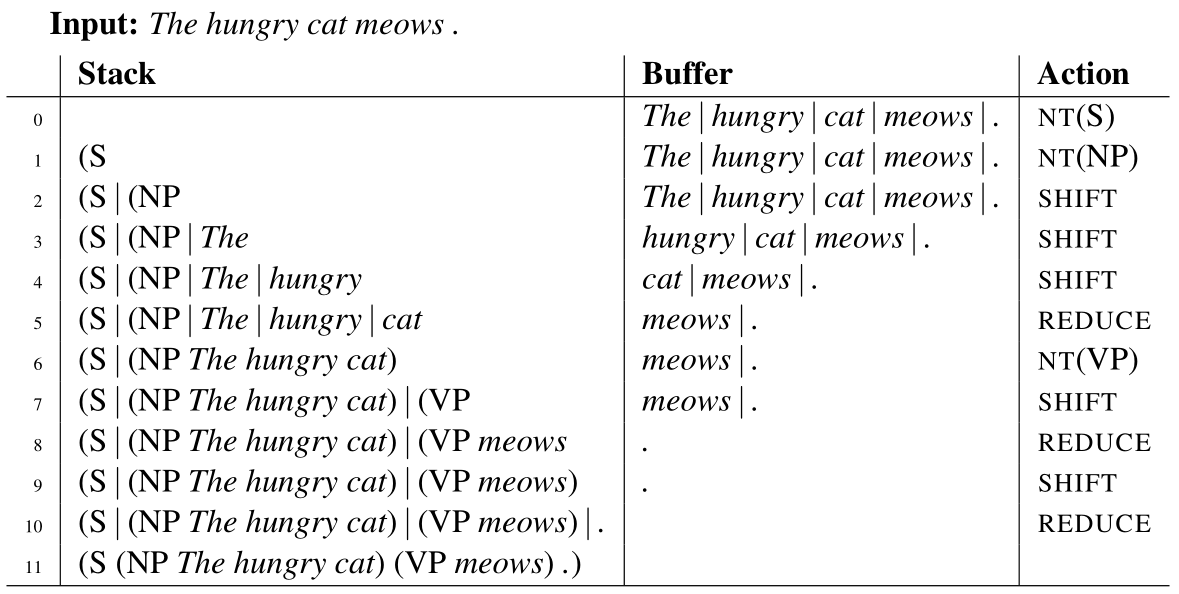
\includegraphics[width=\textwidth]{fig/fig_2.png}
    \end{figure}
  \end{block}
\end{frame}

\begin{frame}{提案手法}
  \begin{block}{構文解析のアルゴリズム}
    \begin{figure}
      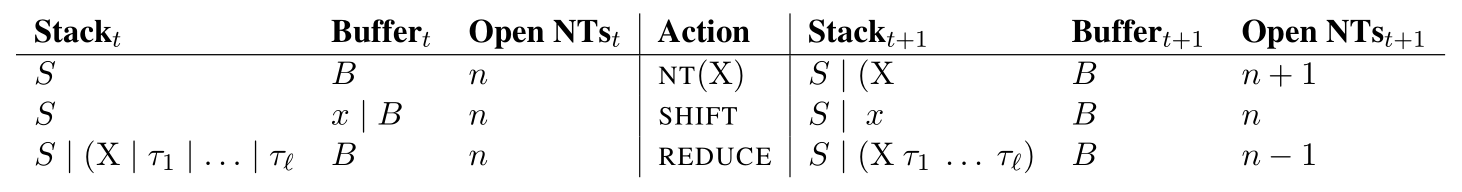
\includegraphics[width=0.95\textwidth]{fig/fig_1.png}
    \end{figure}
    \vspace{-1.75ex} % HACK
    \begin{figure}
      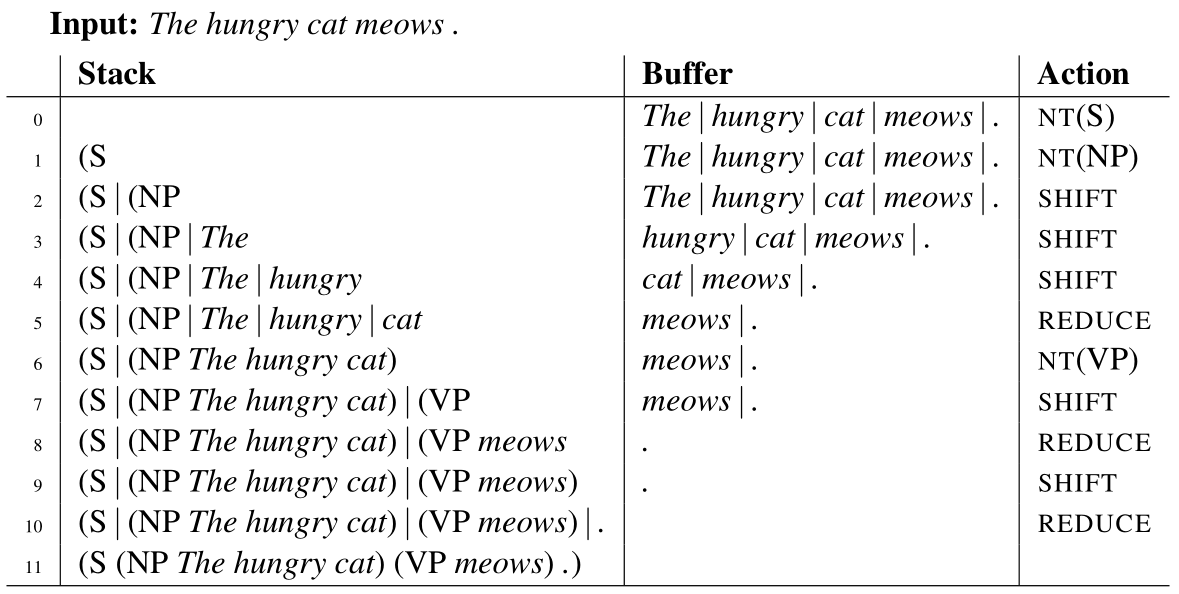
\includegraphics[width=0.95\textwidth]{fig/fig_2.png}
    \end{figure}
  \end{block}
\end{frame}

\begin{frame}<presentation:0>{提案手法}
  \begin{block}{文生成のアルゴリズム}
    \begin{figure}
        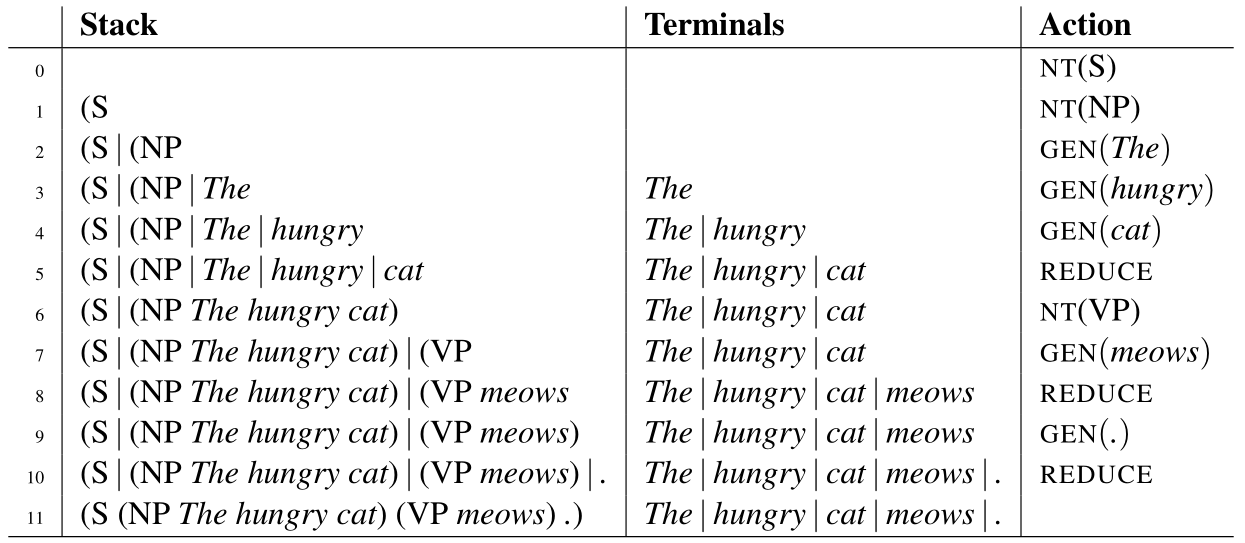
\includegraphics[width=\textwidth]{fig/fig_4.png}
    \end{figure}
  \end{block}
\end{frame}

\begin{frame}{提案手法}
  \begin{block}{文生成のアルゴリズム}
    \begin{figure}
        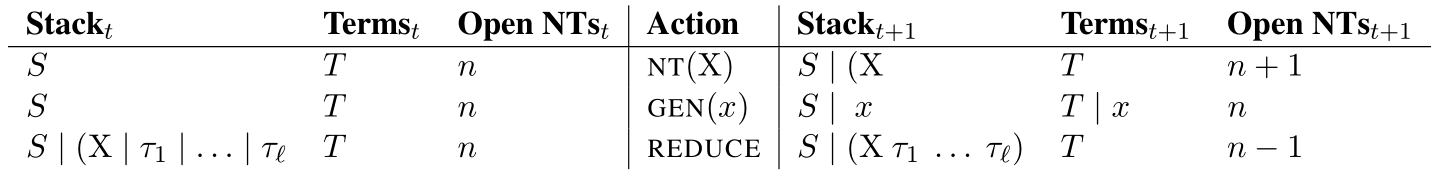
\includegraphics[width=\textwidth]{fig/fig_3.png}
    \end{figure}
    \vspace{-1ex} % HACK
    \begin{figure}
        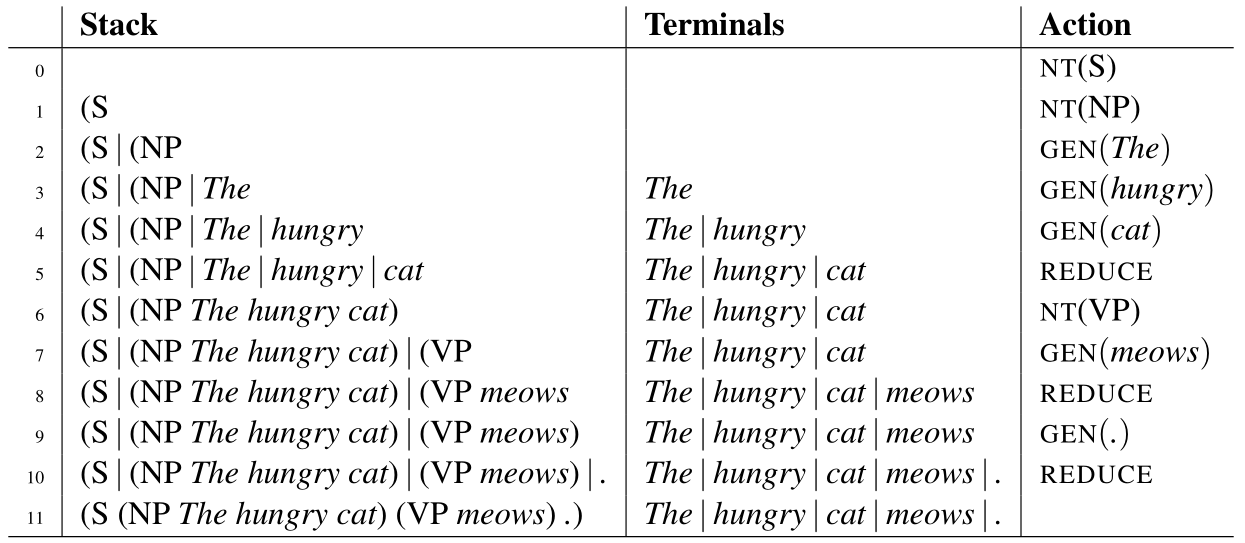
\includegraphics[width=\textwidth]{fig/fig_4.png}
    \end{figure}
  \end{block}
\end{frame}

\begin{frame}{提案手法}
  \begin{block}{生成モデル}
    \begin{itemize}
      \item 最大化: $p(X, Y; \Theta)$
      \item 単語列$\mb{x}$と構文木$\mb{y}$の結合確率
    \end{itemize}
    \begin{gather*}
      p(\mb{x}, \mb{y}) = \prod_{t=1}^{|\mb{a}(\mb{x}, \mb{y})|}
                          p(a_t | \mb{a}_{<t}) \\
      p(a_t | \mb{a}_{<t})
      = \frac{\exp (\mb{r}_{a_t}^T \mb{u}_t + b_{a_t})}
        {\sum_{a' \in A_G(T_t, S_t, n_t)}
         \exp (\mb{r}_{a'}^T \mb{u}_t + b_{a'})} \\
      \begin{cases}
        \mb{a}(x, y): \text{単語列$x$と構文木$y$に対応する行動の列} \\
        \mb{u}_t: \text{アルゴリズムの状態を表す埋め込み} \\
        \mb{r}_a: \text{生成器の各行動の埋め込み(パラメータ)} \\
        b_a: \text{生成器の各行動のバイアス(パラメータ)} \\
      \end{cases}
    \end{gather*}
  \end{block}
\end{frame}

\begin{frame}{提案手法}
  \begin{block}{生成モデル}
    \begin{itemize}
      \item $\mb{u}_t$: アルゴリズムの状態を表す埋め込み
    \end{itemize}
    \begin{align*}
      \mb{u}_t & = \tanh (\mb{W}[\mb{o}_t; \mb{s}_t; \mb{h}_t] + \mb{c})
    \end{align*}
    \begin{gather*}
      \begin{cases}
        \mb{o}_t: \text{出力バッファの状態を表す埋め込み} \\
        \mb{s}_t: \text{スタックの状態を表す埋め込み} \\
        \mb{h}_t: \text{行動履歴を表す埋め込み} \\
        \mb{W}, \mb{c}: \text{パラメータ}
      \end{cases}
    \end{gather*}
  \end{block}
\end{frame}

\begin{frame}{提案手法}
  \begin{block}{生成モデル}
    \begin{itemize}
      \item スタック・出力バッファ・行動履歴内の要素の埋め込みを\\エンコード
    \end{itemize}
    \begin{figure}
      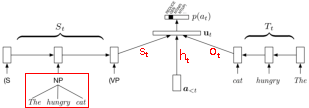
\includegraphics[width=\textwidth]{fig/fig_5.pdf}
    \end{figure}
    \begin{itemize}
      \item スタック内の非終端記号の埋め込みは?
    \end{itemize}
  \end{block}
\end{frame}

\begin{frame}{提案手法}
  \begin{block}{生成モデル}
    \begin{itemize}
      \item Syntactic Composition Function
        \begin{itemize}
          \item REDUCE時に要素の埋め込みから\\その\nt の埋め込みを生成
        \end{itemize}
    \end{itemize}
    \begin{figure}
      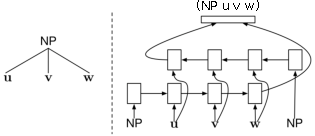
\includegraphics[width=0.8\textwidth]{fig/fig_6.pdf}
    \end{figure}
  \end{block}
\end{frame}

\begin{frame}{提案手法}
  \begin{block}{識別モデル}
    \begin{itemize}
      \item 最大化: $p(Y | X; \Theta)$
      \item 生成モデルの出力バッファ$T$を入力バッファ$B$に置き換え
      \item 単語列$\mb{x}$が与えられているため、 \\
            先ほどの$p(\mb{x}, \mb{y})$を$p(\mb{y}|\mb{x})$として学習
    \end{itemize}
  \end{block}
\end{frame}

\begin{frame}{提案手法}
  \begin{block}{生成モデルにおける重点サンプリング}
    \begin{itemize}
      \item 提案分布$q(\mb{y}|\mb{x})$:識別モデルを利用
      \item 重要度重み:$w(\mb{x}, \mb{y}) = p(\mb{x}, \mb{y}) / q(\mb{y} | \mb{x})$
      \item $\mb{y}$を$q$からサンプリングしモンテカルロ法で計算
      \item 言語モデル
        \begin{align*}
          p(\mb{x})
          & = \sum_{\mb{y} \in \mathcal{Y}(\mb{x})} p(\mb{x}, \mb{y}) \\
          & = \sum_{\mb{y} \in \mathcal{Y}(\mb{x})} q(\mb{y}|\mb{x}) w(\mb{x}, \mb{y}) \\
          & = E_{q(\mb{y}|\mb{x})} w(\mb{x}, \mb{y})
        \end{align*}
      \item 構文解析
        \begin{gather*}
          \hat{\mb{y}} = \mathrm{argmax}_{\mb{y} \sim q(\mb{y}|\mb{x})} p(\mb{x}, \mb{y})
        \end{gather*}
    \end{itemize}
  \end{block}
\end{frame}

\begin{frame}{実験}
  \begin{block}{実験設定}
    \begin{itemize}
      \item データセット
        \begin{itemize}
          \item Penn Treebank(英語)
          \item Penn Chinese Treebank(中国語)
        \end{itemize}
      \item タスク
        \begin{itemize}
          \item 構文解析(生成・識別モデル)
          \item 言語モデル(生成モデル)
        \end{itemize}
    \end{itemize}
    % \begin{figure}
    %   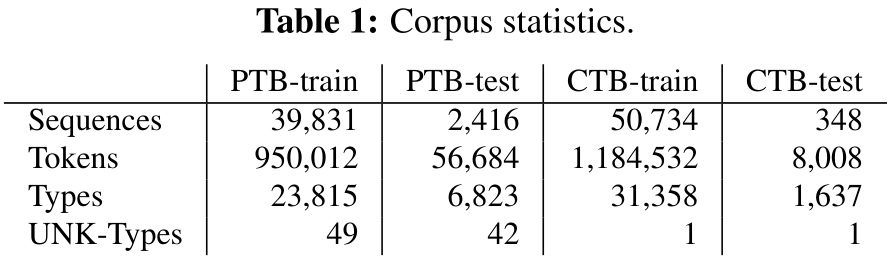
\includegraphics[width=0.8\textwidth]{fig/tab_1.png}
    % \end{figure}
  \end{block}
\end{frame}

\begin{frame}{実験}
  \begin{block}{Penn TreebankでのF値}
    \begin{figure}
      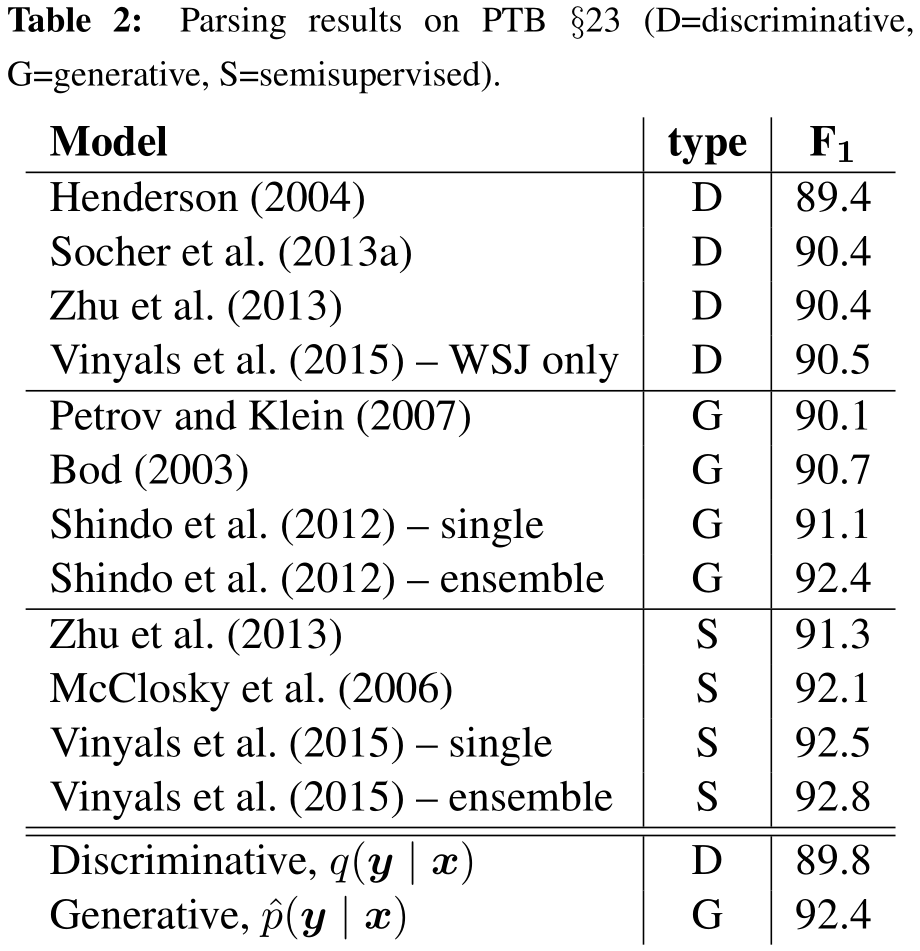
\includegraphics[width=0.575\textwidth]{fig/tab_2.png}
    \end{figure}
  \end{block}
\end{frame}

\begin{frame}{実験}
  \begin{block}{Penn Chinese TreebankでのF値}
    \begin{figure}
      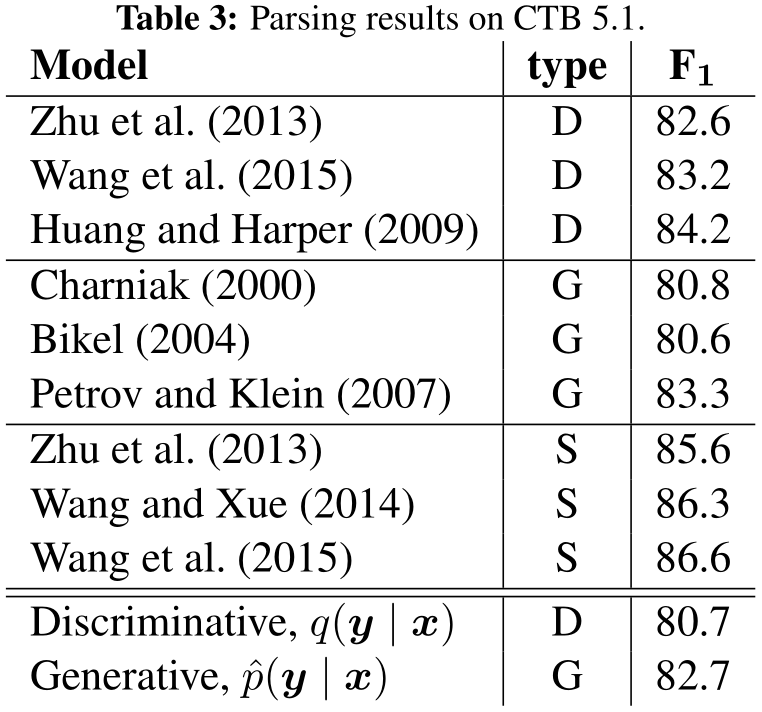
\includegraphics[width=0.45\textwidth]{fig/tab_3.png}
    \end{figure}
    \vspace{-1em}
    \begin{itemize}
      \item 識別モデルの方が生成モデルより性能低い
      \item 大きく構造化されていない条件付きの文脈は \\
            識別モデルにとって学習が難しい
    \end{itemize}
  \end{block}
\end{frame}

\begin{frame}{実験}
  \begin{block}{言語モデルのperplexity}
    \begin{figure}
      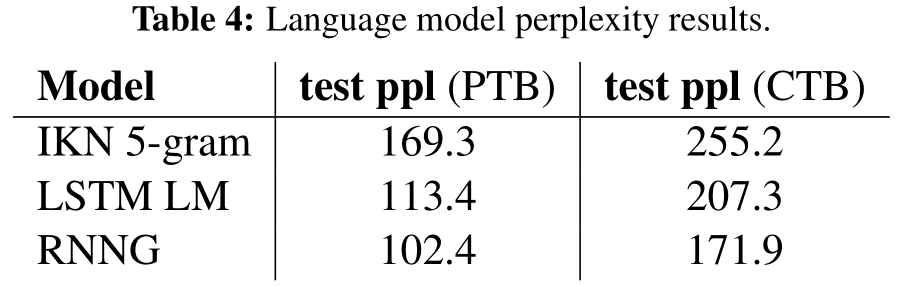
\includegraphics[width=0.7\textwidth]{fig/tab_4.png}
    \end{figure}
  \end{block}
\end{frame}

\begin{frame}{まとめ}
  \begin{itemize}
    \item RNNによる文法のモデルを提案
    \item 遷移ベースの構文解析・文生成アルゴリズムで学習
    \item 生成モデルと識別モデルの2種類
    \item State-of-the-artな手法と同等の性能
    % \item 特徴量の設計やTreebankデータの変換が要らない
  \end{itemize}
\end{frame}

\begin{frame}{感想}
  \begin{itemize}
    \item 構文解析はよく知らなかったので勉強になった
    \item 文法をNNでモデル化しようという発想が面白いと思った
    \item スタックのエンコードがsequentialの場合との比較が知りたい
  \end{itemize}
\end{frame}

\begin{frame}
  \centering \large 補足資料
\end{frame}

\begin{frame}{提案手法}
  \begin{block}{構文解析のアルゴリズム}
    \begin{gather*}
      \begin{cases}
        x: \text{\term (単語)の列(入力)} \\
        y: \text{構文木(出力)} \\
        S: \text{スタック} \\
        B: \text{入力バッファ}
      \end{cases}
    \end{gather*}
    \begin{itemize}
      \item スタックの要素:\term、openまたはclosedな\nt
      \item 入力バッファの要素:\term
      \item 初期状態
        \begin{gather*}
          \begin{cases}
            S = \emptyset \\
            B = [T_1, \ldots, T_n] \\
          \end{cases}
        \end{gather*}
    \end{itemize}
  \end{block}
\end{frame}

\begin{frame}{提案手法}
  \begin{block}{構文解析のアルゴリズム}
    \begin{figure}
      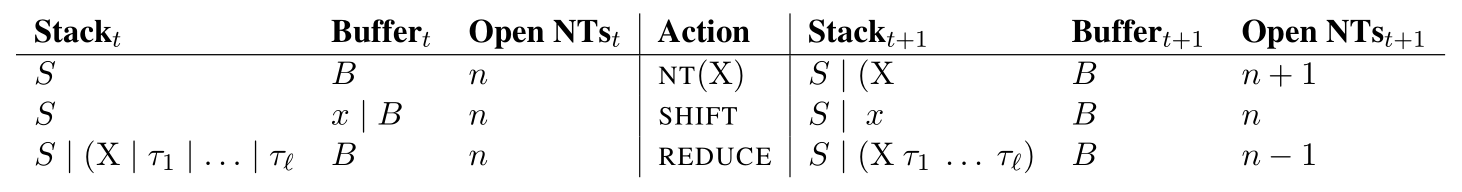
\includegraphics[width=\textwidth]{fig/fig_1.png}
    \end{figure}
    \begin{itemize}
      \item 遷移の制約
        \begin{itemize}
          \item $n$: スタック内の\opennt の数
        \end{itemize}
        \begin{table}
          \begin{tabular}{c | l}
            遷移 & 制約 \\
            \hline
            NT(X)   & $B \neq \emptyset \wedge n < 100$ \\
            \hline
            SHIFT   & $B \neq \emptyset \wedge n \geq 1$ \\
            \hline
            REDUCE  & \parbox{20em}{$
              \text{スタック内の一番上の要素が} \\
              \text{\opennt でない} \\
              \wedge (n \geq 2 \vee B = \emptyset)
            $} \\
          \end{tabular}
        \end{table}
    \end{itemize}
  \end{block}
\end{frame}

\begin{frame}{提案手法}
  \begin{block}{文生成のアルゴリズム}
    \begin{gather*}
      \begin{cases}
        x: \text{\term (単語)の列\fire{(出力)}} \\
        y: \text{構文木(出力)} \\
        S: \text{スタック} \\
        \fire{T: \text{出力バッファ}}
      \end{cases}
    \end{gather*}
    \begin{itemize}
      \item スタックの要素:\term、openまたはclosedな\nt
      \item 出力バッファの要素:\term
      \item 初期状態
        \begin{gather*}
          \begin{cases}
            S = \emptyset \\
            T = \emptyset \\
          \end{cases}
        \end{gather*}
    \end{itemize}
  \end{block}
\end{frame}

\begin{frame}{提案手法}
  \begin{block}{文生成のアルゴリズム}
    \begin{figure}
      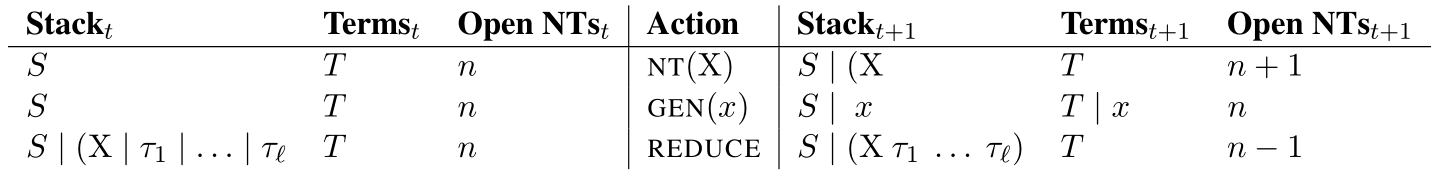
\includegraphics[width=\textwidth]{fig/fig_3.png}
    \end{figure}
    \begin{itemize}
      \item 遷移の制約
        \begin{itemize}
          \item $n$: スタック内の\opennt の数
        \end{itemize}
        \begin{table}
          \begin{tabular}{c | l}
            遷移 & 制約 \\
            \hline
            GEN(X) & $n \geq 1$ \\
            \hline
            REDUCE  & \parbox{20em}{$
              \text{スタック内の一番上の要素が} \\
              \text{\opennt でない} \\
              \wedge n \geq 1
            $} \\
          \end{tabular}
        \end{table}
    \end{itemize}
  \end{block}
\end{frame}

\begin{frame}{提案手法}
  \begin{block}{生成モデルにおける単語の推定}
    \begin{itemize}
      \item Class-factored softmax
        \begin{itemize}
          \item $|\Sigma|$:語彙数
          \item Brown et al., 2016の手法により語彙を \\
                $\sqrt{|\Sigma|}$個のクラスタに分割
          \item 単語の推定の計算量:$O(\sqrt{|\Sigma|})$
        \end{itemize}
        \begin{gather*}
          p(x) = p(x|c)p(c)
        \end{gather*}
    \end{itemize}
  \end{block}
\end{frame}

\end{document}
